\documentclass[a4paper]{report} % Formato plantilla

\usepackage{graphicx}
\usepackage[utf8]{inputenc} % Para poder usar caracteres especiales
\usepackage[spanish]{babel} % Para poder usar caracteres especiales

\begin{document} % Inicio del documento Template
  \begin{titlepage}
    \centering
    {\scshape\LARGE Universidad Católica de Pereira\par}
    \vfill
    {\scshape\LARGE Redes de Datos 2\par}
    \vfill
    {\huge\bfseries Apuntes de clase\par}
    \vfill
    {\Large\itshape Juan David Garcia Acevedo\par}
    \vfill
    Docente de la materia\par
	  Rafael Ricardo \textsc{Rubiano}
    \vfill
    {\Large\today\par}
  \end{titlepage}
%======================================================================
  \tableofcontents % Para crear los índices
    \part{Introducción al Enrutamiento de Red}
      \chapter{Repaso Introducción a las Redes}
        \section{Redes de Datos}
          \subsection{Conceptos Básicos} 
            \paragraph{Repaso}\mbox{} \\
              Las redes al día de hoy conectan al mundo, siendo \textbf{CISCO} quien liderea este mundo (Salud, Estudio, Medicina y todos los contextos), todo esta en la red.
              Es importante recordar que una red de computadoras es donde dos \textit{Hosts} están comunicandose entre si (recordar que un \textbf{Host} es todo dispositivo con tarjeta de red).
              \\\\Las redes son las que permiten el viaje de la información.
              \begin{itemize}
                \item Ventajas
                  \begin{enumerate}
                    \item Fácil configurar
                    \item Menos complejo
                    \item Reduce costos
                    \item Tareas simples
                  \end{enumerate}
                \item Desventajas
                  \begin{enumerate}
                    \item No esta centralizada la administración
                    \item No son seguras
                    \item No son escalables
                    \item Rendimiento lento
                  \end{enumerate}
              \end{itemize}
              Recordar los \textit{Routers} como intermediarios de comunicación, y los medios de red como los elementos por donde viaja la información.
              \begin{table}[t]
                \begin{center}
                  \begin{tabular}{| r | l | c |}
                    \centering
                      Tipos de medio & Descripción & Uso \\ \hline
                    Alambres de metal dentro del cable & Pulsos electricos & Confiabilidad \\
                      Fibras de vidrio o plastico & Pulsos de luz & Seguridad \\
                      Transmisión Inalambrica & Modulación de frecuencias & Mobilidad \\ \hline
                  \end{tabular}
                  \caption{Medios de red}
                  \label{tab:medios}
                \end{center}
              \end{table}
              Los protocolos permiten que haya una comunicación entre \textbf{Tx} y \textbf{Rx}.
              \\\\En el cuadro \ref{tab:medios} veremos los tipos de medios usados para transmitir la información por la red, descripción y uso.
%=====================================================================
            \subsection{Tipos comunes de redes}
              \paragraph{Redes}\mbox{} \\
                Aunque las redes más comunes son las redes Lan y Wan, hay otro tipo de redes
%---------------------------------------------------------------------
            \subsection{Protocolos y Modelos}
%---------------------------------------------------------------------
            \subsection{Modelo OSI}
%---------------------------------------------------------------------
            \subsection{Conceptos Enrutamiento de Red}
              \paragraph{¿Qué es enrutamiento de red?}\mbox{} \\
                Para que dos redes puedan comunicarse entre sí es necesaria la existencia de un dispositivo intermediario que tenga la capacidad de transmitir los paquetes de unas redes a otras. Esto lo hacen mediante los \textbf{Routers}.
                \\La función principal de los \textbf{Routers} es la de buscar el mejor camino, entre los posibles, hacia un destino para dirigir el tráfico hacia él. Esto se logra mediante \textit{Tablas de Enrutamiento} que contienen la información sobre las redes que están conectadas directamente al router, además de las rutas hacia otras redes.
%---------------------------------------------------------------------
        \section{Introducción Enrutamiento de Red}
          \subsection{Protocolos}
            \subsubsection{TCP}
            \subsubsection{UDP}
            \subsubsection{SCTP}
              \paragraph{}\mbox{} \\
          \subsection{Diferencias TCP vs UDP}
%---------------------------------------------------------------------
          \subsection{Enrutamiento Estático}
            \paragraph{}\mbox{} \\
              El enrutamiento estático es aquel en el que el administrador de la red debe encargarse de configurar manualmente cada uno de los enrutadores que forman la red. Para la correcta configuración el administrador debe manualmente configurar enrutador por enrutador, uno a uno configurar y enseñarle las rutas existentes.
              \\Este tipo de enrutamiento hace más fácil el mantenimiento de las \textit{Tablas de Enrutamiento} en redes muy pequeñas, en las cuales no se presente a futuro una escalabilidad en la red.
              \\\\Podemos concluir que, el \textbf{Enrutamiento Estático} se utiliza principalmente en redes con una cantidad pequeña de enrutadores, las cuales tienen un solo \textit{Gateway o Puerta de enlace}. Cuando se lleva a cabo este tipo de configuración, hay que especificar en cada router la IP de destino, la IP del router por la que se envían los paquetes, la distancia y la máscara de red.
%---------------------------------------------------------------------
          \subsection{Enrutamiento Dinámico}
            \paragraph{}\mbox{} \\
              El enrutamiento dinámico se basa en la utilización o empleo de protocolos de enrutamiento con el fin de automatizar el intercambio y la actualización de las tablas de enrutamiento de cada uno de los routers. Estos protocolos comparten las tablas de enrutamiento de forma automática con los routers cercanos, lo que hace que su utilización sea recomendada para redes grandes.
              \\Si tenemos una red en la que utilizamos este tipo de enrutamiento, no importará la cantidad de routers que contenga, ya que podremos ir agregando en ella nuevos equipos y automáticamente todos los routers los conocerán sin necesidad de configurar cada uno de ellos de forma individualizada. Todo es automático, por ejemplo, si elimino una red WAN o LAN todos los equipos sabrán que no existe y no enviarán paquetes a la misma. O si por el contrario, la agrego, todos la conocerán y podrán comunicarse con ella.
              \\Es fundamental comprender que, en este caso, los routers se comunican unos a otros las redes a las que están conectados, lo que lo hace mucho más rápido y eficiente.
            \subsubsection{Estado Enlace}
              \paragraph{}\mbox{}\\
                \\\\Podemos concluir que el \textbf{Estado Enlace} elige la mejor ruta dependiendo del estado de los enlaces, solo de los estados están encendidos.

            \subsubsection{Vector Distancia}
              \paragraph{}\mbox{}\\
                \begin{figure}[htb]
                  \centering
                    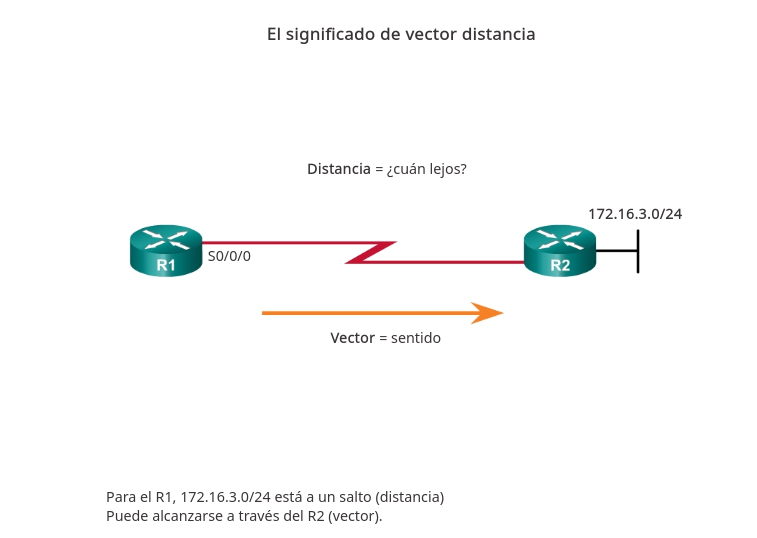
\includegraphics[width=\textwidth]{Images/vector-distancia.png}
                      \caption{Ejemplo del vector distancia}
                      \label{fig:vector-distancia}
                \end{figure}
              \\Podemos concluir que el \textbf{Vector Distancia} es dferente, puesto este no se fia por los enlaces encendidos, sino por el peso del ancho de banda, ya que estos tienen los enlace más grandes.
              \\Si el enlace se cae, no supone un problema puesto, este se recalcula de manera automatica.
%----------------------------------------------------------------------
    \part{Protocolo de Internet}
    \part{Calidad de servicios y Control de Tráfico}
    \part{Tecnología MPLS}
    \part{Voz sobre paquetes}
    \part{Seguridad en Redes IP}
    \part{Tecnologías de acceso a Banda Ancha}
%----------------------------------------------------------------------
    \part{Metodología de Calificación}
      \chapter{Cortes}
        \section{Porcentajes evaluativos}
          \paragraph{Cortes 1, 2, 3}\mbox{}\\
            \begin{itemize}
              \item Corte 1
              \begin{enumerate}
                \item Talleres 10\%
                \item Proyecto 10\%
                \item Parcial 15\%
                \item Acumulado 35\%
              \end{enumerate}
              \item Corte 2
              \begin{enumerate}
                 \item Talleres 10\%
                \item Proyecto 10\%
                \item Parcial 15\%
                \item Acumulado 35\%
              \end{enumerate}
              \item Corte 3
              \begin{enumerate}
                \item Talleres 10\%
                \item Proyecto 10\%
                \item Parcial 15\%
                \item Acumulado 35\%
              \end{enumerate}
            \end{itemize}
%======================================================================
\end{document}

